% Group meeting, 2026-08-17 — Keheng Zhu
% Release path only: the Saha closure and the 1600 km truncation, the SWMF
% exact-Riemann Godunov flux, a short note on a storage-precision fix, and the
% upper-boundary conduction-wall temperature sensitivity.
%
% Scope note: this deck deliberately presents ONLY the release path. The
% equilibrium-Gamma1 Roe reference flux, the Roe-vs-Godunov comparison and the
% CFL signal-speed audit are not on these slides; the full record lives in
% docs/studies/numerics/swmf_godunov_flux_experiment.md.
%
% Build (keeps aux files out of the source directory):
%   cd docs/presentations/2026-08-17-group-meeting
%   latexmk -pdf -output-directory=build presentation.tex
%
% Every number traces to a file named on the backup "Sources" frame.
\documentclass[aspectratio=169]{beamer}

\usetheme{AnnArbor}          % Michigan maize & blue, as in the 2026-07-11 talk
\usecolortheme{rose}
\useinnertheme{rectangles}
\setbeamertemplate{navigation symbols}{}
\setbeamerfont{frametitle}{size=\normalsize}
\setbeamertemplate{itemize items}[circle]
\setbeamertemplate{blocks}[rounded]

\usepackage{amsmath,amssymb}
\usepackage{graphicx}
\usepackage{booktabs}
\usepackage{xcolor}

% Figures live in this talk's own figures/ directory so the deck builds from a
% fresh clone; visualization/ is gitignored. See figures/README.md.
\graphicspath{{figures/}}

\newcommand{\src}[1]{{\scriptsize\color{gray}#1}}
\definecolor{f32}{RGB}{214,39,40}
\definecolor{f64}{RGB}{31,119,180}

\title[Release numerics update]{Release numerics update}
\subtitle{The ionization closure, the domain, the new face solver, and how much
          the top boundary matters}
\author{Keheng Zhu}
\institute{University of Michigan}
\date{17 August 2026}

\begin{document}

\begin{frame}
  \titlepage
\end{frame}

% ============================================================ roadmap
\begin{frame}{Where we are}
  \vfill
  \begin{columns}[T]
    \begin{column}{0.60\textwidth}
      \begin{enumerate}
        \item Which ionization closure, and where can we trust it?
        \item[]
        \item A new face solver: the SWMF exact Riemann problem.
        \item[]
        \item {\color{gray}A precision fix, briefly.}
        \item[]
        \item How much does the \emph{top} boundary set the answer?
      \end{enumerate}
    \end{column}
    \begin{column}{0.38\textwidth}
      \footnotesize
      \textbf{The release model}\\[4pt]
      1.5D field-aligned single fluid\\[2pt]
      $U=(\rho,\ \rho u,\ E)$\\[6pt]
      Saha equilibrium EOS\\[2pt]
      MUSCL--Hancock $\rightarrow$ Godunov\\[2pt]
      $\rightarrow$ implicit conduction\\[6pt]
      1600--2153\,km, 661 cells
    \end{column}
  \end{columns}
  \vfill
\end{frame}

% ============================================================ A. ionization
\section{Ionization closure and the domain}

\begin{frame}{What sets hydrogen ionization in the chromosphere?}
  \begin{columns}[c]
    \begin{column}{0.61\textwidth}
      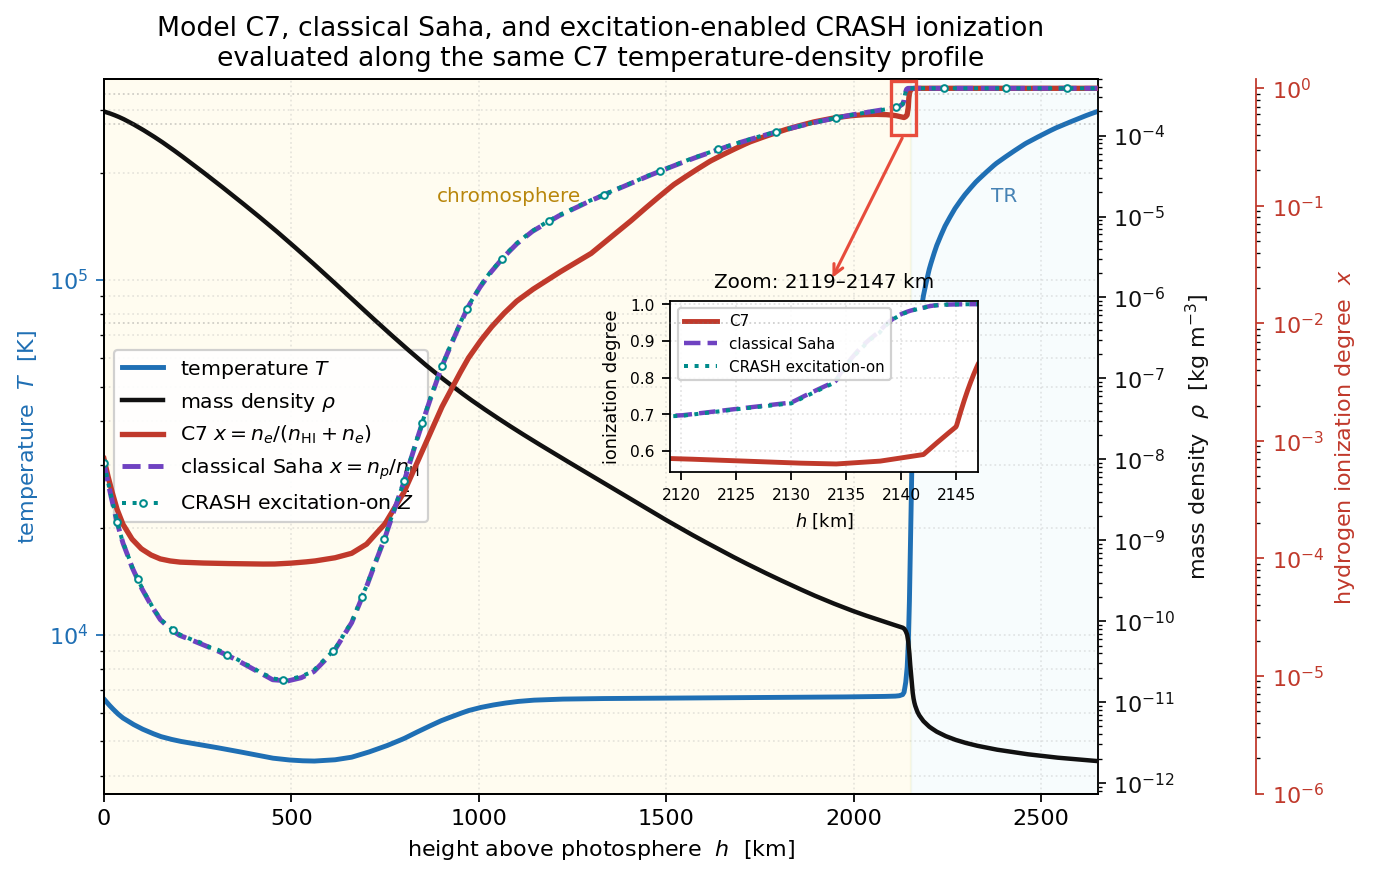
\includegraphics[width=\textwidth]{c7_ionization_profile_compare.png}
    \end{column}
    \begin{column}{0.37\textwidth}
      \footnotesize
      \begin{itemize}\itemsep8pt
        \item Above $\sim$1.8\,Mm, Saha \textbf{tracks} the semi-empirical C7.
              Both cross $x=0.5$ within 7\,km.
        \item Lower down they part --- and the \textbf{sign flips}: C7 is
              $10\times$ higher at 500\,km, $3\times$ lower at 1200\,km.
        \item Excitation physics does \textbf{not} close the gap.
      \end{itemize}
    \end{column}
  \end{columns}
  \vspace{4pt}
  \src{\hfill C7 is non-LTE (Avrett \& Loeser 2008); the other curves are LTE
       equilibrium on C7's own $(T,n_{\rm H})$.}
\end{frame}

\begin{frame}{Two consequences}
  \vfill
  \begin{columns}[T]
    \begin{column}{0.47\textwidth}
      \textbf{We adopt Saha equilibrium}
      \vspace{6pt}
      \begin{itemize}\itemsep6pt
        \item One consistent, differentiable closure: $x$, $n_e$, $p$,
              $e_{\rm int}$ from $(\rho,T)$.
        \item $x$ is \textbf{derived} --- never stored, never advanced.
        \item Ionization energy is carried in $e_{\rm int}$.
      \end{itemize}
    \end{column}
    \begin{column}{0.47\textwidth}
      \textbf{We truncate at 1600\,km}
      \vspace{6pt}
      \begin{itemize}\itemsep6pt
        \item A mid-chromospheric reservoir --- \alert{not the photosphere}.
        \item Where we stop claiming the closure applies. Below is
              \emph{outside the model}.
        \item Quasi-static, stratified, $v=0$.
      \end{itemize}
    \end{column}
  \end{columns}
  \vfill
  \begin{center}\footnotesize
    \color{gray} 1600\,km is a judgement call, not a derived height.
  \end{center}
\end{frame}

% ============================================================ B. Godunov
\section{The release face solver}

\begin{frame}{The release face solver: SWMF exact Riemann}
  \textbf{Ported, not reinvented:}
  \vspace{2pt}
  \begin{itemize}\footnotesize\itemsep1pt
    \item \texttt{SWMF/util/CRASH/src/test\_godunov.f90} :: \texttt{get\_godunov\_flux}
    \item \texttt{SWMF/share/Library/src/ModExactRS.f90} ::
          \texttt{exact\_rs\_pu\_star}, \texttt{exact\_rs\_sample}
  \end{itemize}
  \vspace{10pt}
  The Saha internal energy \textbf{splits exactly}:
  \vspace{-2pt}
  \begin{equation*}
    e_{\rm int} \;=\;
      \underbrace{\frac{p}{5/3-1}}_{\text{monatomic translation}}
      \;+\;
      \underbrace{e_{\rm ion}}_{\text{rides in the offset } E_0}
  \end{equation*}
  \vspace{2pt}
  \begin{center}
    \textbf{Split $\rightarrow$ solve $\rightarrow$ sample $\rightarrow$ carry $E_0$}
  \end{center}
\end{frame}

\begin{frame}{Split $\rightarrow$ solve $\rightarrow$ sample $\rightarrow$ carry}
  \vfill
  \begin{enumerate}\itemsep10pt
    \item \textbf{Split.} Translational gas at $\gamma=5/3$; ionization energy
          and gravitational potential into an offset
          $E_0=\bigl(E-\tfrac12\rho u^2-p/(\gamma-1)\bigr)/\rho$.
    \item \textbf{Solve} the local \emph{ideal-gas} Riemann problem exactly.
    \item \textbf{Sample} the self-similar solution at $x/t=0$.
    \item \textbf{Carry $E_0$} with the contact, then rebuild the energy flux.
  \end{enumerate}
  \vfill
  \begin{block}{Why freezing composition is the right limit}
    Chromospheric hydrogen cannot re-equilibrate on a wave timescale:
    $\tau_{\rm ion}\sim10^5$\,s in the mid-chromosphere, still $10$--$10^3$\,s
    inside shocks --- against a dynamical time of $\sim$1\,minute.
    \src{Carlsson \& Stein 2002; Leenaarts+ 2007, 2020}
  \end{block}
\end{frame}

\begin{frame}{Verification}
  \vfill
  \begin{itemize}\itemsep10pt
    \item Toro's \textbf{five standard tests}, to the 6 published digits.
    \item Degenerate cases \emph{exact}: a stationary contact carries
          identically zero mass.
    \item $E_0$ verified to advect passively --- no effect beyond round-off.
    \item 4000\,s production run: \textbf{941\,679\,108 faces, all solved
          exactly, zero fallbacks.}\\
          \src{Release validation now fails on a nonzero fallback count.}
  \end{itemize}
  \vfill
  \begin{center}\footnotesize
    \color{gray} The bulk EOS is still Saha equilibrium. Composition is frozen
    only \emph{across the wave interaction} --- this is not a finite-rate
    ionization model.
  \end{center}
\end{frame}

% ============================================================ C. precision
\section{A precision fix}

\begin{frame}{Aside: the lower-chromosphere mass flux was a storage bug}
  \begin{columns}[c]
    \begin{column}{0.44\textwidth}
      \footnotesize
      Continuity: a quasi-steady column must carry a \textbf{height-independent}
      mass flux. Ours did not.
      \vspace{10pt}
      \[ \rho \mathrel{+}= \Delta t\cdot\mathrm{rhs} \]
      \vspace{-6pt}

      In \textbf{619 of 660 cells} that increment is below half a float32 ULP of
      $\rho$ --- it rounds straight back. The density cannot respond.
      \vspace{12pt}

      {\color{gray}A double-precision control, everything else identical, makes
      it flat. Not physics, not the solver, not the boundary. It is \emph{not}
      cosmetic: top-of-domain evaporation drops $\sim$28\% (13.18 $\rightarrow$
      9.50\,m/s), so every float32-era evaporation number was high.}
    \end{column}
    \begin{column}{0.52\textwidth}
      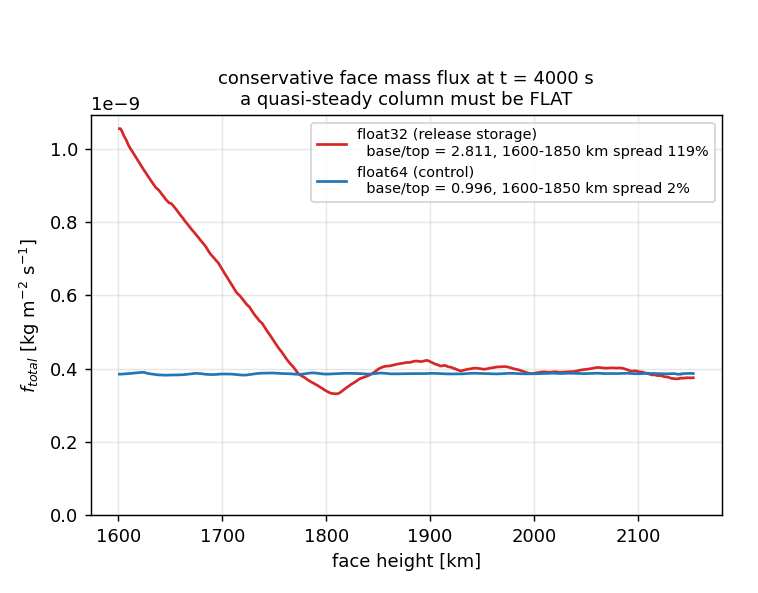
\includegraphics[width=\textwidth]{precision_ftotal_4000s.png}
    \end{column}
  \end{columns}
\end{frame}

% ============================================================ D. upper boundary
\section{The upper boundary}

\begin{frame}{How much does the top boundary set the answer?}
  \begin{columns}[c]
    \begin{column}{0.55\textwidth}
      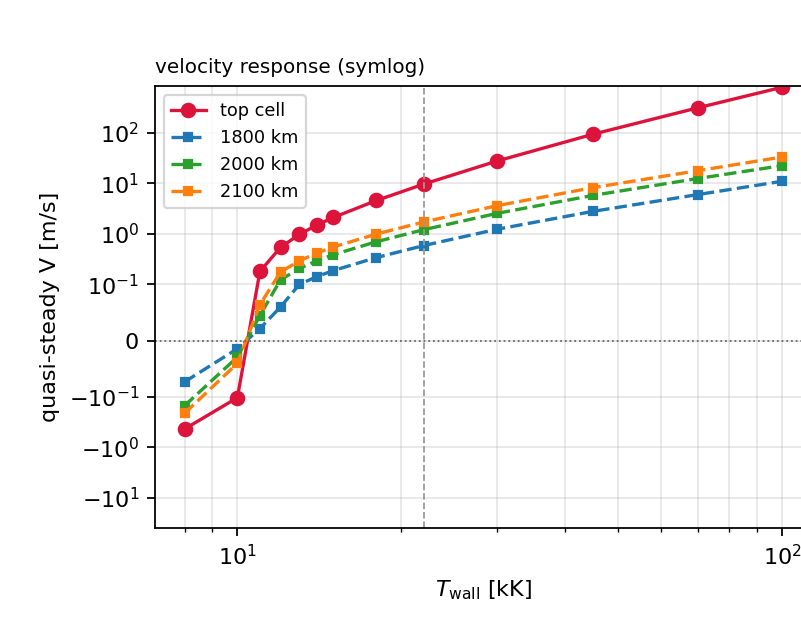
\includegraphics[width=\textwidth]{twall_response.png}
    \end{column}
    \begin{column}{0.43\textwidth}
      \footnotesize
      \textbf{One knob: $T_{\rm wall}$ at the 2153\,km face.}
      \vspace{4pt}

      8, 10, 11, 12, 13, 14, 15, 18,\\
      \textbf{22}, 30, 45, 70, 100\,kK
      \vspace{2pt}

      \src{13 runs $\times$ 4000\,s. Same C7 start, everything else fixed.}
      \vspace{10pt}
      \begin{itemize}\itemsep8pt
        \item $-0.4 \rightarrow +792$\,m/s.\\
              \textbf{Four decades of $V$ per decade of $T_{\rm wall}$.}
        \item Reverses near 10\,kK: the column \textbf{drains}, not evaporates.
        \item \alert{Local slope 3.7 at our 22\,kK.}\\
              10\% in the wall $\Rightarrow$ 40\% in the evaporation.
      \end{itemize}
    \end{column}
  \end{columns}
  \vspace{2pt}
  \src{\hfill $\rho V$ flat to 14\% in height: a mass-flux response. $V(h)$
       rises only because $\rho$ falls.}
\end{frame}

\begin{frame}{Conduction sets it; ionization pays for it}
  \begin{columns}[c]
    \begin{column}{0.47\textwidth}
      \footnotesize
      \textbf{Three links, all measured:}
      \vspace{6pt}
      \begin{enumerate}\itemsep7pt
        \item \textbf{Thermostat.} $T_{\rm top}$ tracks $T_{\rm wall}$ to 0.3\%,
              so $\Delta T \propto T_{\rm wall}^{0.8}$ --- self-limiting.
        \item \textbf{Spitzer.} $\kappa\propto T^{2.50}\ \Rightarrow\
              q_{\rm wall}\propto T_{\rm wall}^{3.3}$.\\
              \src{All the nonlinearity. Mach $\le0.015$.}
        \item \textbf{Export.} No radiative sink, so\\
              $V \simeq q_{\rm wall}/[\rho_{\rm top}(h + x\chi_H/m_H)]$.
      \end{enumerate}
    \end{column}
    \begin{column}{0.51\textwidth}
      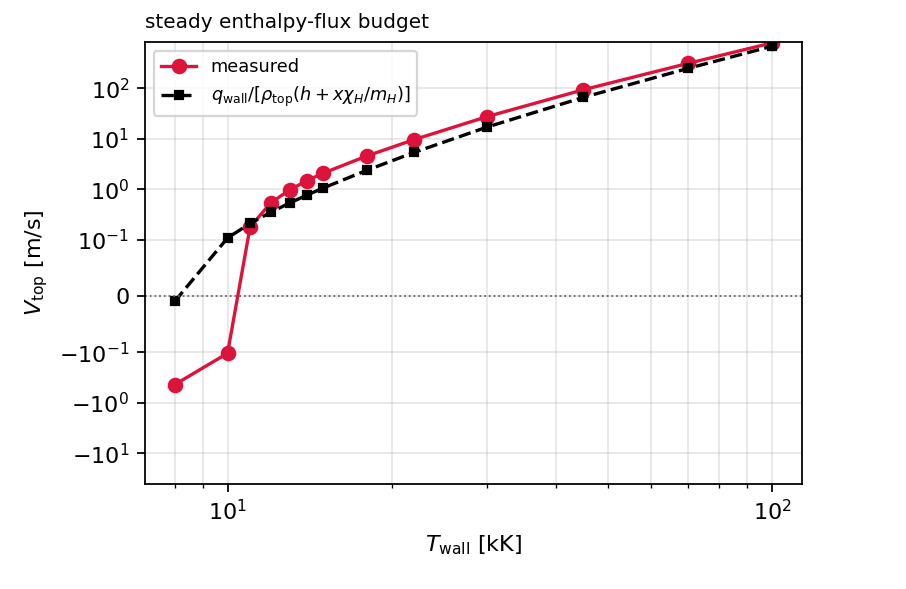
\includegraphics[width=\textwidth]{twall_enthalpy_budget.png}
    \end{column}
  \end{columns}
  \vspace{-2pt}
  \begin{center}\footnotesize
    Within a factor of two across four decades, no fitting.
    \alert{Ionization is 59\% of that denominator at 22\,kK.}
  \end{center}
\end{frame}

% ============================================================ status
\section{Status}
\begin{frame}{Status and open questions}
  \begin{center}\footnotesize
    \color{gray}Release: single-fluid Saha equilibrium mixture; MUSCL--Hancock +
    SWMF exact Riemann; implicit conduction; 107 test cases green.
  \end{center}
  \vfill
  \begin{enumerate}\itemsep11pt
    \item \textbf{Saha vs.\ finite relaxation.} Composition frozen \emph{inside}
          the Riemann problem, re-equilibrated \emph{after every step}.\\
          Finite-rate network, or a relaxation source?
    \item \textbf{The top boundary is the dominant lever.} $V\propto
          T_{\rm wall}^{3}$.\\
          Couple to a real corona, or keep quoting a chosen wall?
    \item \textbf{Resolution.} N500 evaporation mass flux: not established as
          $<$10\% grid-converged.
    \item \textbf{Minor, tracked.} One artifact at the first interior face ---
          survives the precision control, so it is real.
  \end{enumerate}
  \vfill
\end{frame}

% ============================================================ backup
\appendix

\begin{frame}{Backup: what the wall sweep does \emph{not} establish}
  \begin{columns}[c]
    \begin{column}{0.46\textwidth}
      \footnotesize
      \begin{itemize}\itemsep8pt
        \item \textbf{Quasi-steady, not steady.} $V_{\rm top}$ still falling
              2--6\% per 500\,s --- magnitudes are upper bounds, the trend is
              not.
        \item \textbf{Reversal bracketed at 8--11\,kK}, not pinned.
        \item \textbf{6\,kK is outside the model:} the top cools below the
              $\Gamma_1$ table floor and aborts.
        \item \textbf{100\,kK needed CFL 0.25.} Matched 70\,kK control:
              $2.6\times10^{-5}$.
        \item \textbf{Back-pressure fixed} --- only the thermal BC moves.
      \end{itemize}
    \end{column}
    \begin{column}{0.52\textwidth}
      % near-square crop: size it by height, or it overflows the frame
      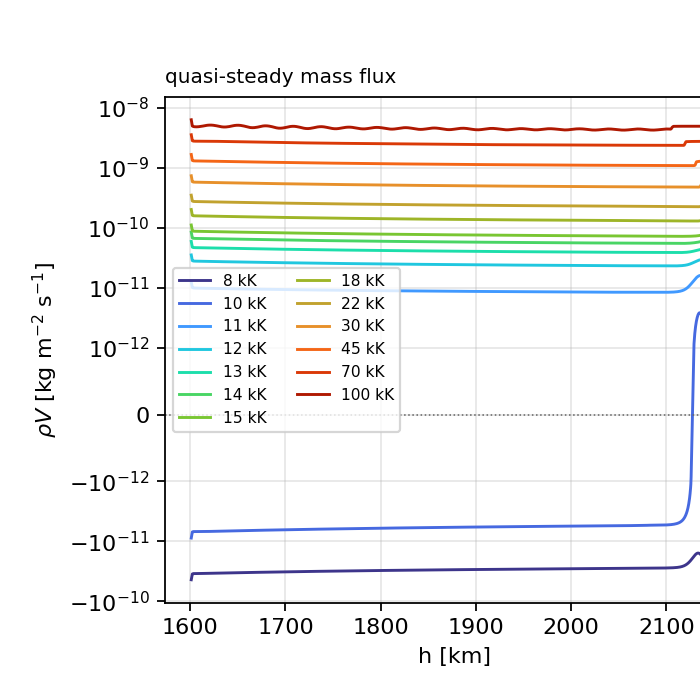
\includegraphics[height=0.66\textheight]{twall_massflux_uniform.png}
      \vspace{-2pt}
      \begin{center}
        \src{$\rho V$ flat with height: a real steady mass flux.}
      \end{center}
    \end{column}
  \end{columns}
\end{frame}

\begin{frame}{Backup: sources}
  \scriptsize
  \begin{tabular}{ll}
    \toprule
    Claim & Where it comes from \\
    \midrule
    C7 vs Saha vs CRASH ionization & \texttt{util/plot\_c7\_ionization\_profile.py --mode compare} \\
    1600\,km truncation & \texttt{docs/doxygen/pages/physics\_model.md}; \texttt{scenarios/model\_column.cpp} \\
    Relaxation timescales & Carlsson \& Stein 2002; Leenaarts et al.\ 2007; Leenaarts 2020 \\
    Toro tests, $E_0$ passivity, 0 fallbacks & \texttt{tests/chromo\_tests.cpp}; \\
      & \texttt{docs/studies/numerics/swmf\_godunov\_flux\_experiment.md} \\
    float32 vs float64 control & \texttt{docs/studies/numerics/float32\_precision\_control\_experiment.md}; \\
      & \texttt{docs/studies/numerics/state\_precision\_release\_cutover.md} \\
    Wall-temperature sweep & \texttt{docs/studies/boundaries/upper\_wall\_temperature\_sensitivity\_recap.md}; \\
      & \texttt{util/run\_twall\_sweep.sh}, \texttt{util/twall\_sweep\_diag.py} \\
    Figure provenance & \texttt{figures/README.md}; \texttt{visualize\_commands.md} \S14--16 \\
    Test counts & \texttt{./build\_omp/chromo\_tests}, current tree \\
    \bottomrule
  \end{tabular}
  \vspace{12pt}
  \begin{center}
    Flux cutover: \texttt{022ea34}\quad$\cdot$\quad
    Reference-free release: \texttt{34ecb00}\quad$\cdot$\quad
    Precision cutover: \texttt{78109a9}\quad$\cdot$\quad
    Wall sweep: \texttt{030347a}
  \end{center}
\end{frame}

\end{document}
